\chapter{Modelo de Interacción}
 
En este capitulo mostramos las interfaces con las que se van a implementar el sistema, estas pantallas y interfaces diseñadas son directamente en código HTML, para poder adelantar un poco la implementación. 
Estas interfaces se utilizan para poder facilitar el entendimiento de la especificación de los requerimientos explicada con casos de uso.


\begin{figure}[htbp!]
	\begin{center}
	Interfaz de Usuario IU0:Login
	Interfaz necesaria para acceder al sistema.
	Esta Interfaz se muestra apenas se visita la URL:www.Farmacia\_Fracs.com
	En ella el Empleado o el dueño introduce su Correo y su clave para poder			Acceder al sistema y utilizarlo.
		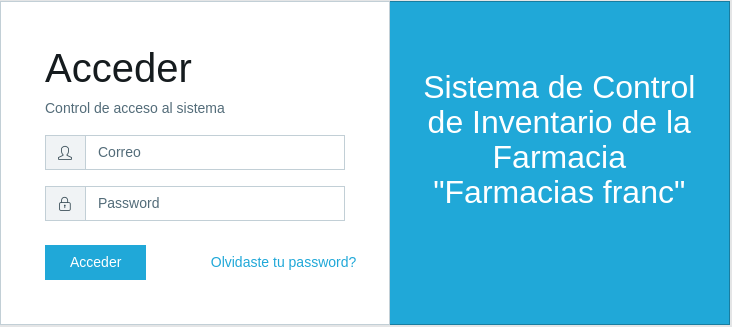
\includegraphics[width=\textwidth]{Pantallas/login}
		\caption{Modelo de interacción}
	\end{center}
\end{figure}



\begin{figure}[htbp!]
	\begin{center}
	
Primera pantalla que se muestra apenas el Empleado o Dueño accede al sistema.
Mostrando un mensaje de bienvenida.
		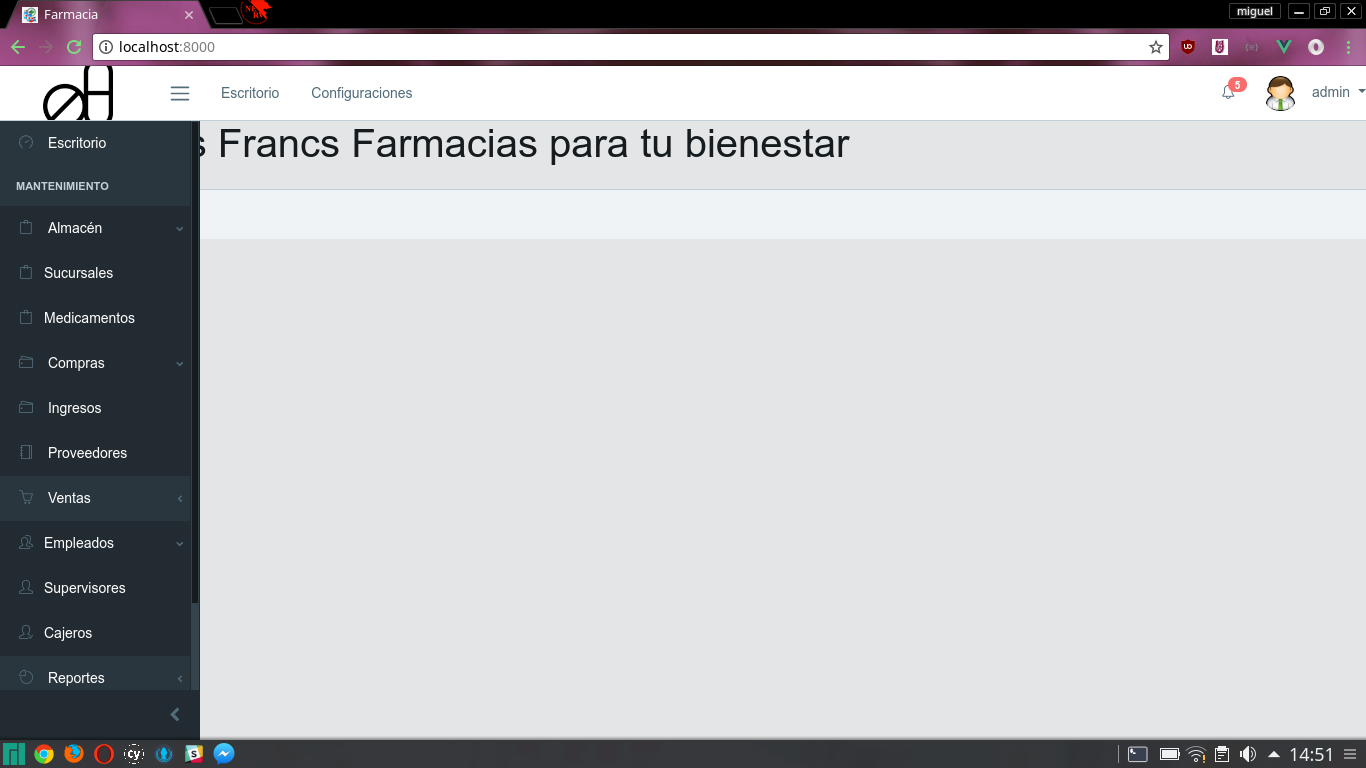
\includegraphics[width=\textwidth]{Pantallas/PantallaPrincipal}
		\caption{Interfaz de Usuario IU1:Pantalla Principal}
	\end{center}
\end{figure}


\begin{figure}[htbp!]
	\begin{center}
	\subsection{Formularios}
	pantallas para mostrar los datos requeridos para agregar un nuevo elemento
y también pantallas que se muestran para actualizar un elemento 
con la diferencia de que los datos estarán llenos.
		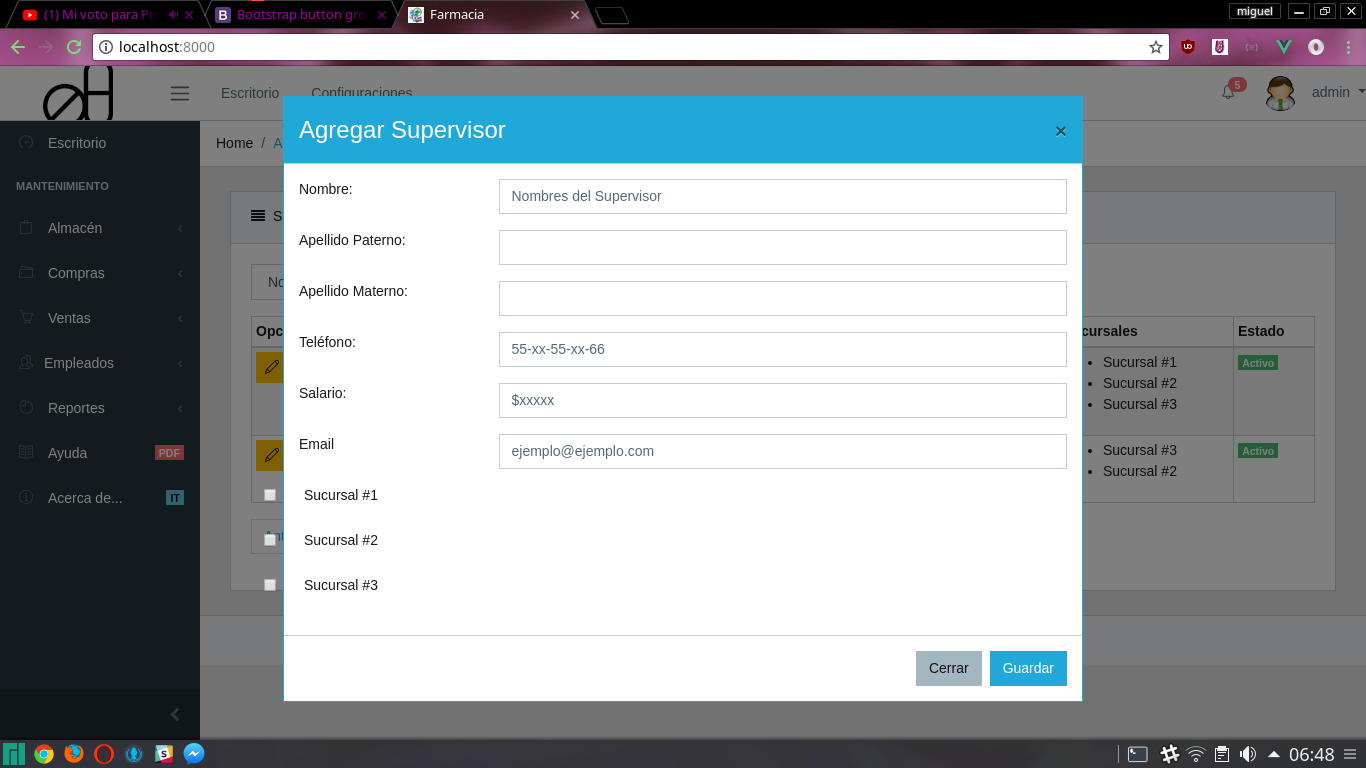
\includegraphics[width=\textwidth]{Pantallas/FormularioSupervisor}
		\caption{Interfaz de Usuario IU2:Formulario Supervisor}
	\end{center}
\end{figure}




\begin{figure}[htbp!]
	\begin{center}
	Pantalla para introducir los datos de la Sucursal que se registra en el sistema.los campos que se muestran en el formulario son: Teléfono de la sucursal, Dirección y el nombre de la sucursal.
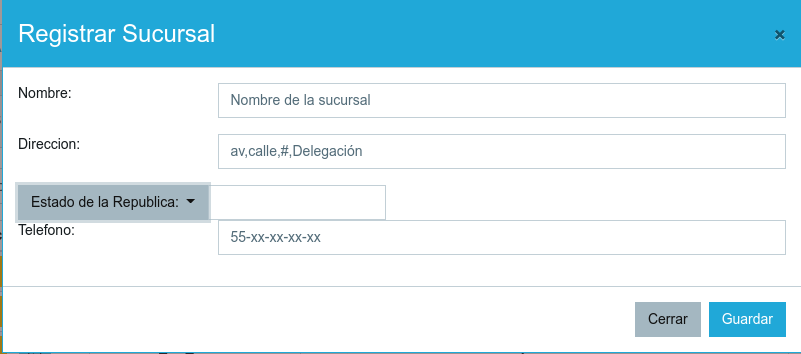
\includegraphics[width=\textwidth]{Pantallas/FormularioSucursal}
		\caption{Interfaz de Usuario IU3: Formulario Sucursal}
	\end{center}
\end{figure}


\begin{figure}[htbp!]
	\begin{center}
	Pantalla que se muestra para Guardar los datos de medicamento.
	Los campos de Lote y fecha de Caducidad vienen en el medicamento.
	El código de barras se llena  utilizando el lector de código de barras.
	los ``select" de los campos ``presentacion" y ``Via de Administración" son catalogos que tienen los atributos que se muestran en el diagrama de clases, en las clases  Presentacion y Via de administracion.
	El laboratorio también esta en la caja del medicamento.
	para guardar los ingredientes activos de un medicamento, se tiene que hacer uno por uno viendo los ingredientes activos que muestra la caja.
	Como el formulario es muy grande se divide en dos imagenes.
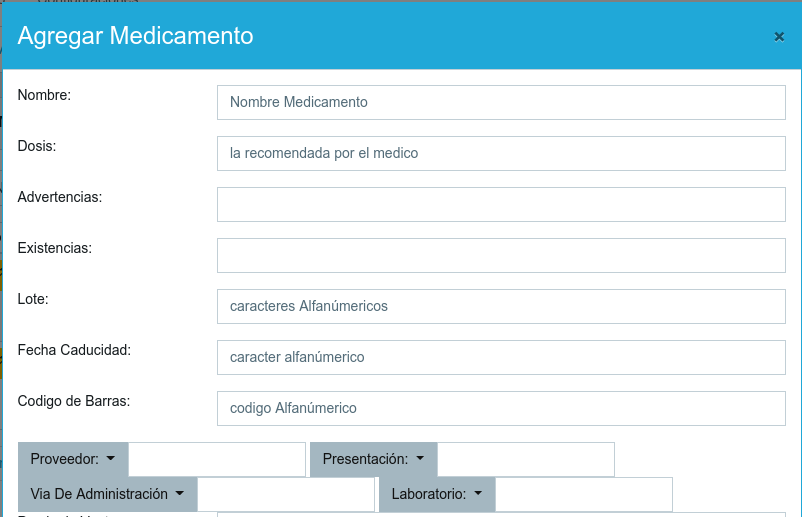
\includegraphics[width=\textwidth]{Pantallas/FormularioMedicamento}
		\caption{Interfaz de Usuario IU5: Formulario Medicamento primera parte}
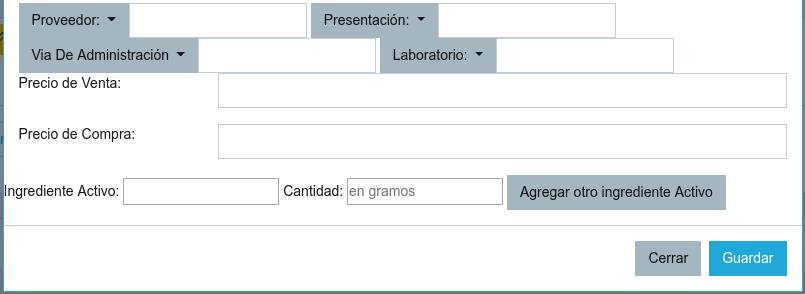
\includegraphics[width=\textwidth]{Pantallas/FormularioMedicamento2}
		\caption{Interfaz de Usuario IU5: Formulario Medicamento segunda parte}
	\end{center}

\end{figure}



\begin{figure}[htbp!]
	\begin{center}
	EN esta pantalla se muestra el formulario de Clientes, En el cual contiene los campos de nombre(s) que hacer referencias a los nombre del cliente, los campos de apellidos paterno y materno, El campo del email es opcional, el campo de Teléfono esta limitado a 40 caracteres en caso de que se anote el número con el carácter ``-" entre cada dos números.
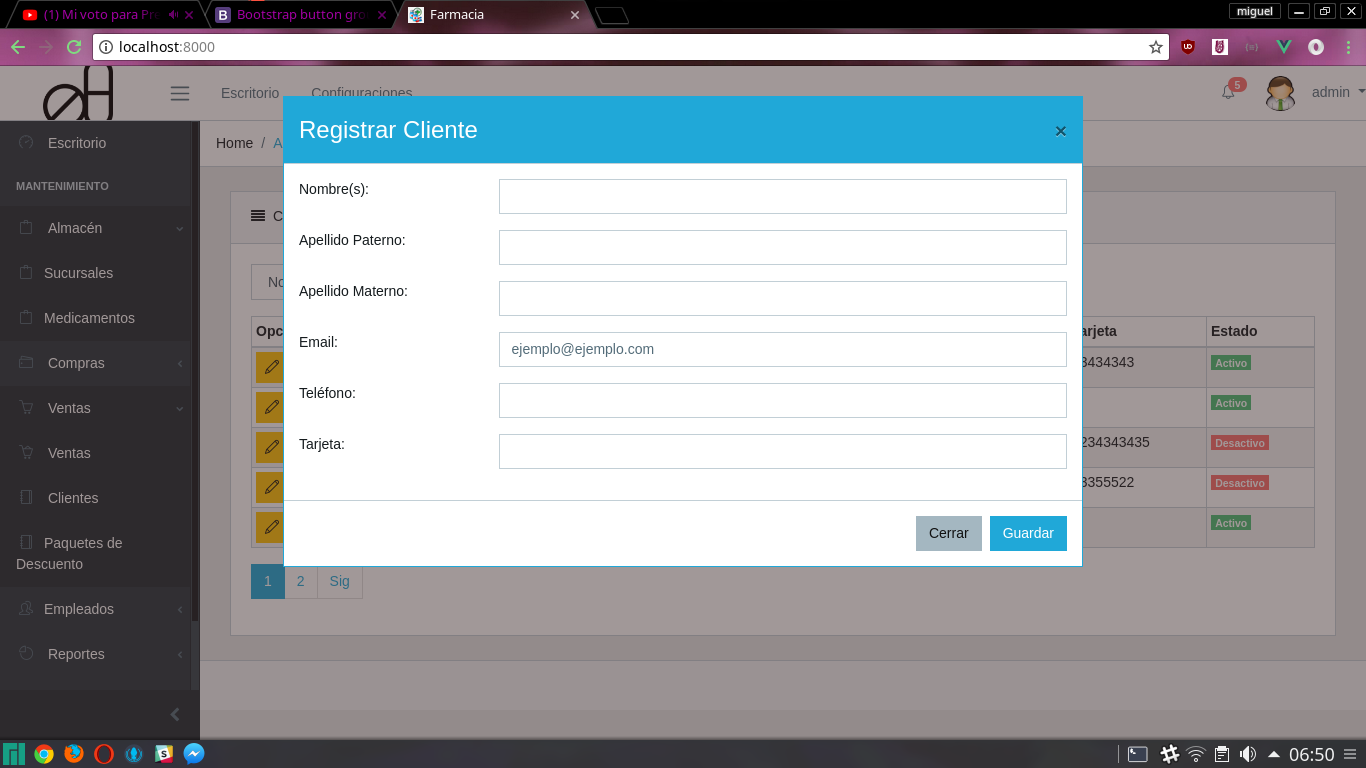
\includegraphics[width=\textwidth]{Pantallas/FormularioClientes}
		\caption{Interfaz de Usuario IU6: Formulario Cliente}
	\end{center}
\end{figure}


\begin{figure}[htbp!]
	\begin{center}
	En esta pantalla se muestra el formulario de agregar cajero, con los campos de nombre, apellido materno, apellido paterno, teléfono y salario. En el campo de Sucursal Se genera una lista desplegable con las sucursales registradas en el sistema.
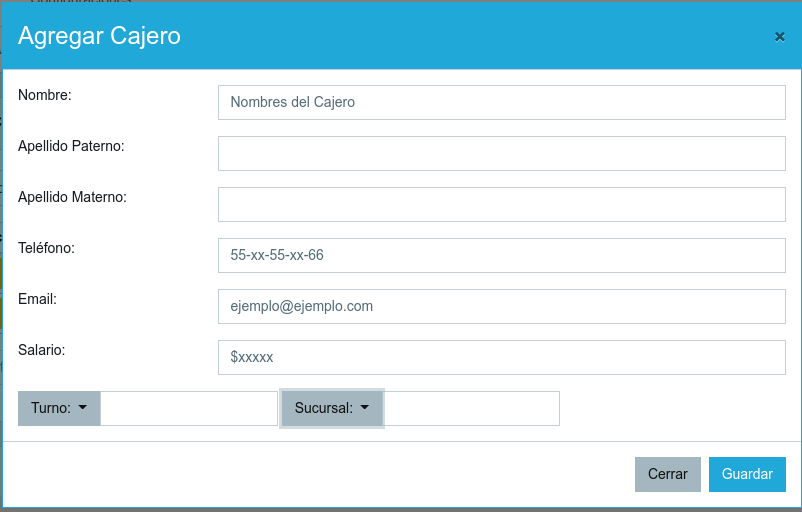
\includegraphics[width=\textwidth]{Pantallas/FormulariCajero}
		\caption{Interfaz de Usuario IU7:Formulario Cajero}
	\end{center}
\end{figure}



\begin{figure}[htbp!]
	\begin{center} 
	En esta pantalla se muestra el formulario para agregar un nuevo proveedor,
	Todos los campos son obligatorios y el campo  de RFC esta limitado a 13 caracteres
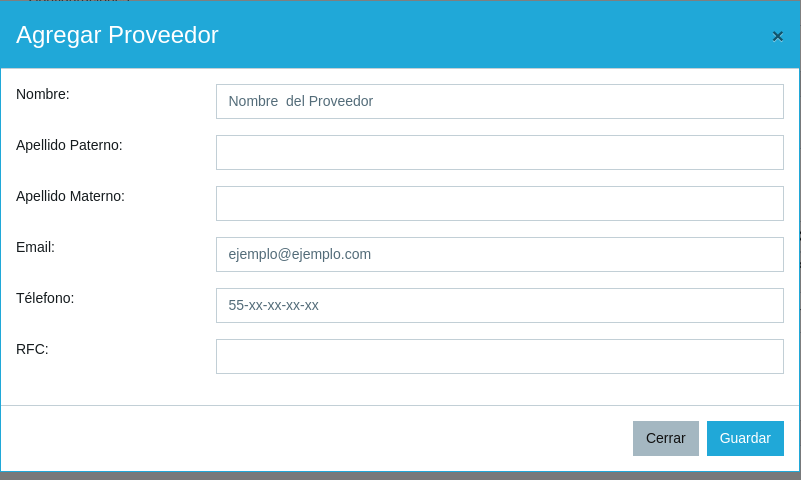
\includegraphics[width=\textwidth]{Pantallas/ProveedorFormulario}
		\caption{Interfaz de Usuario IU8:Formulario Proveedor}
	\end{center}
\end{figure}


\begin{figure}[htbp!]
	\begin{center}
	 \subsection{Botones}
	Botón para poder desactivar a un elemento.

\includegraphics[scale=1]{Pantallas/bottonDesactivar}
		\caption{Interfaz de Usuario IU9:Botón desactivar}
	\end{center}
\end{figure}



\begin{figure}[htbp!]
	\begin{center}
	Botón que se muestra en las opciones de las tablas para poder activar un elemento

\includegraphics[scale=1]{Pantallas/bottonActivar}
		\caption{Interfaz de Usuario IU10:Botón activar}
	\end{center}
\end{figure}



\begin{figure}[htbp!]
	\begin{center}
	\subsection{Tablas}
En estas Interfaces se muestran las tablas con los respectivos datos en formato
de tabla, donde también hay una columna extra aparte de los atributos que tiene el elemento, que muestra las opciones que se tienen para interactuar con los datos
del elemento. En el caso de que el elemento sea Medicamentos, no se muestran todos los atributos ya que son demasiados,por eso en la columna de opciones tiene una opción para ver los demás atributos en la tabla.
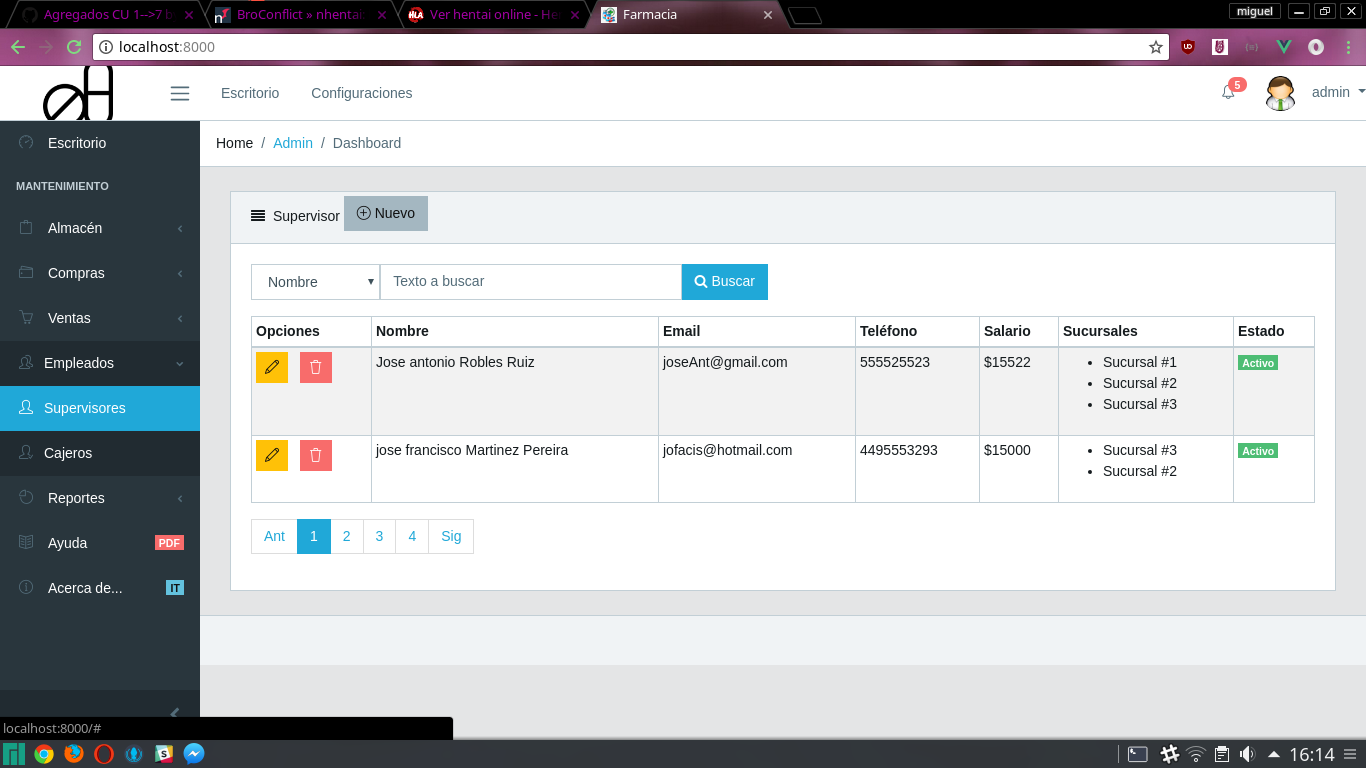
\includegraphics[width=\textwidth]{Pantallas/tablaSupervisores}
		\caption{Interfaz de Usuario IU13:Tabla supervisores.}
	\end{center}
\end{figure}




\begin{figure}[htbp!]
	\begin{center}
	Pantalla donde se muestra un tabla con los datos de la Sucursal.
	en la columna de dirección se agrega el dato del estado de la república con el que se guardo la sucursal, tiene la columna de opciones, tiene una columna para mostrar si la sucursal esta activa o no, y tiene la opción hasta arriba de la tabla de poder buscar una sucursal por el estado o por su nombre.
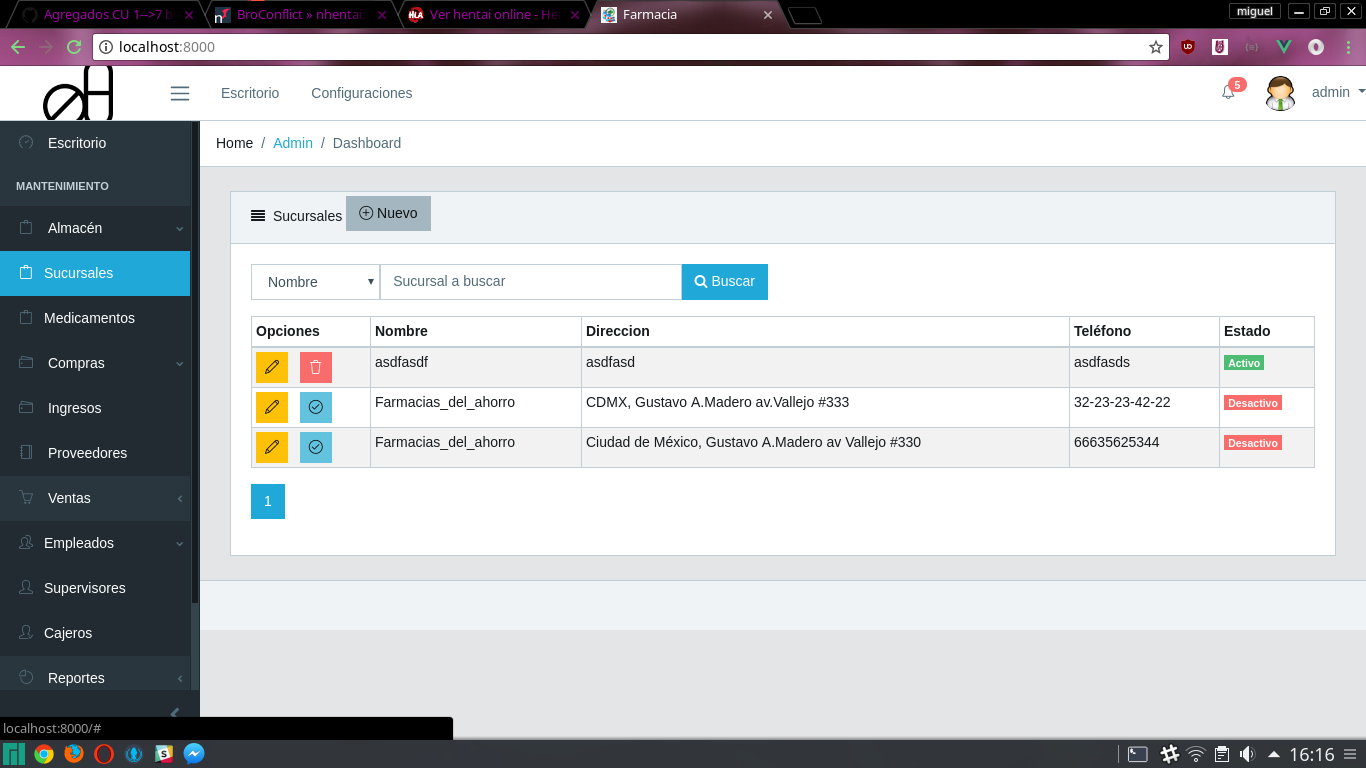
\includegraphics[width=\textwidth]{Pantallas/tablaSucursales}
		\caption{Interfaz de Usuario IU14:Tabla Sucursales.}
	\end{center}
\end{figure}



\begin{figure}[htbp!]
	\begin{center}
	Pantalla donde se muestra la información obtenida del proveedor.
	con las mismas características que todas las tablas,y teniendo en los campos de búsqueda la opción de buscar a un proveedor por su nombre o su RFC
	
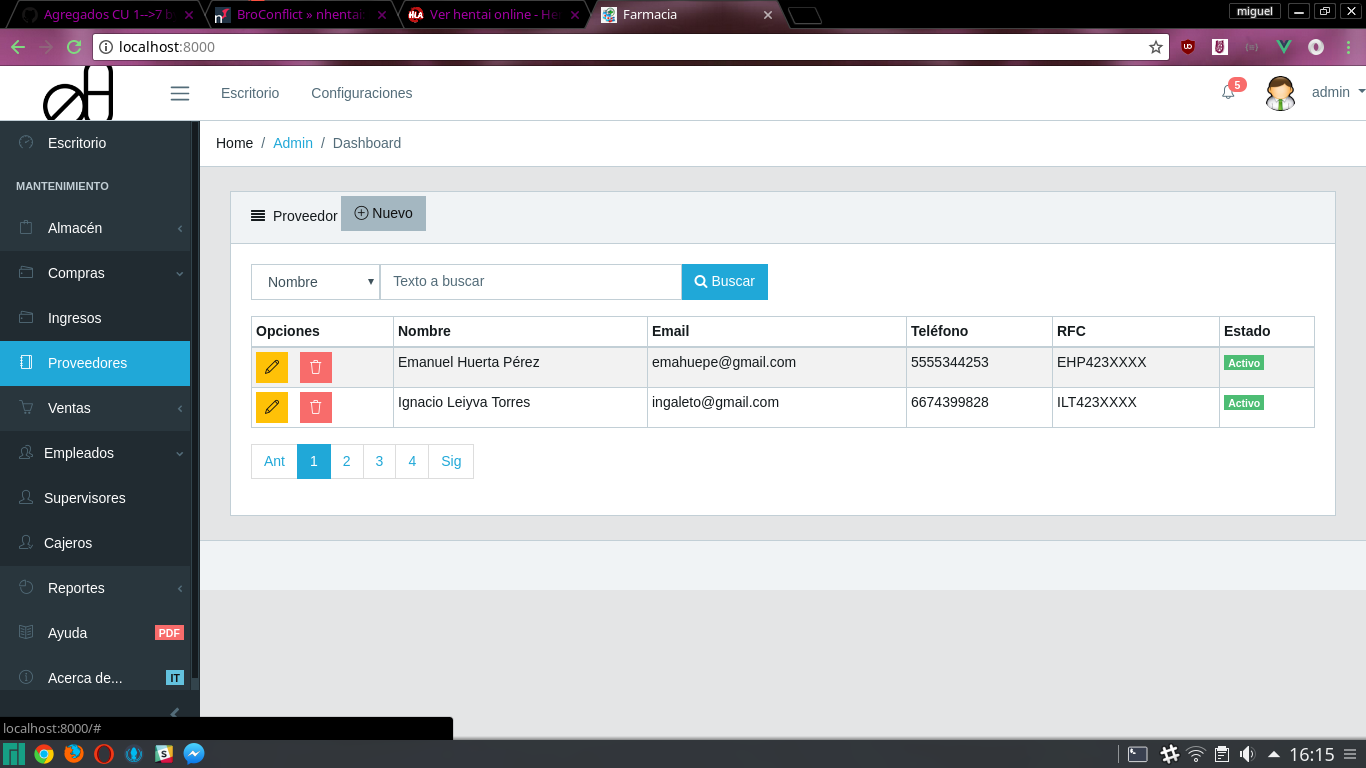
\includegraphics[width=\textwidth]{Pantallas/tablaProveedores}
		\caption{Interfaz de Usuario IU15:Tabla Proveedores.}
	\end{center}
\end{figure}





\begin{figure}[htbp!]
	\begin{center}
	En esta pantalla se tiene la tabla con algunos campos de datos de los medicamentos, no se muestran todos los datos porque estos son demasiados, 
	para poder visualizar todos los datos en la tabla se presiona el botón ``más información" y se desprenden las demás columnas de los datos faltantes:Advertencias, Existencias,  Lote, Fecha Caducidad, código de barras, el proveedor, Presentación, Vía de administración, Laboratorio, Precio Compra e ingrediente activo con su cantidad
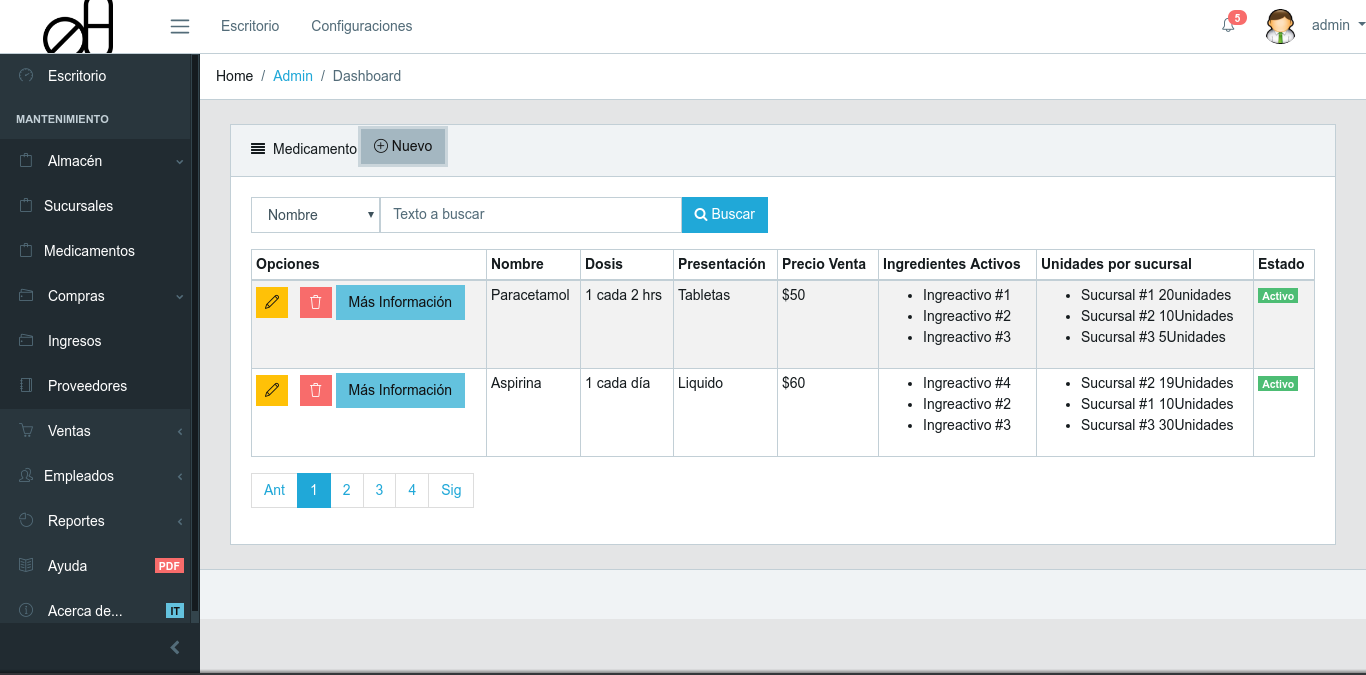
\includegraphics[width=\textwidth]{Pantallas/TablaMedicamentos}
		\caption{Interfaz de Usuario IU17:Tabla Medicamentos.}
	\end{center}
\end{figure}



\begin{figure}[htbp!]
	\begin{center}
	Tabla que muestra la información de un cajero, nombre, email, teléfono, salario, sucursal, turno y estado, muestra las opciones para modificar, activar y desactivar al cajero, aunque la parte de editar a un cajero aun no esta implementada.la información del cajero se muestra en formato de tabla donde los datos del empleado estan en cada columna y los empleados estan en diferentes filas
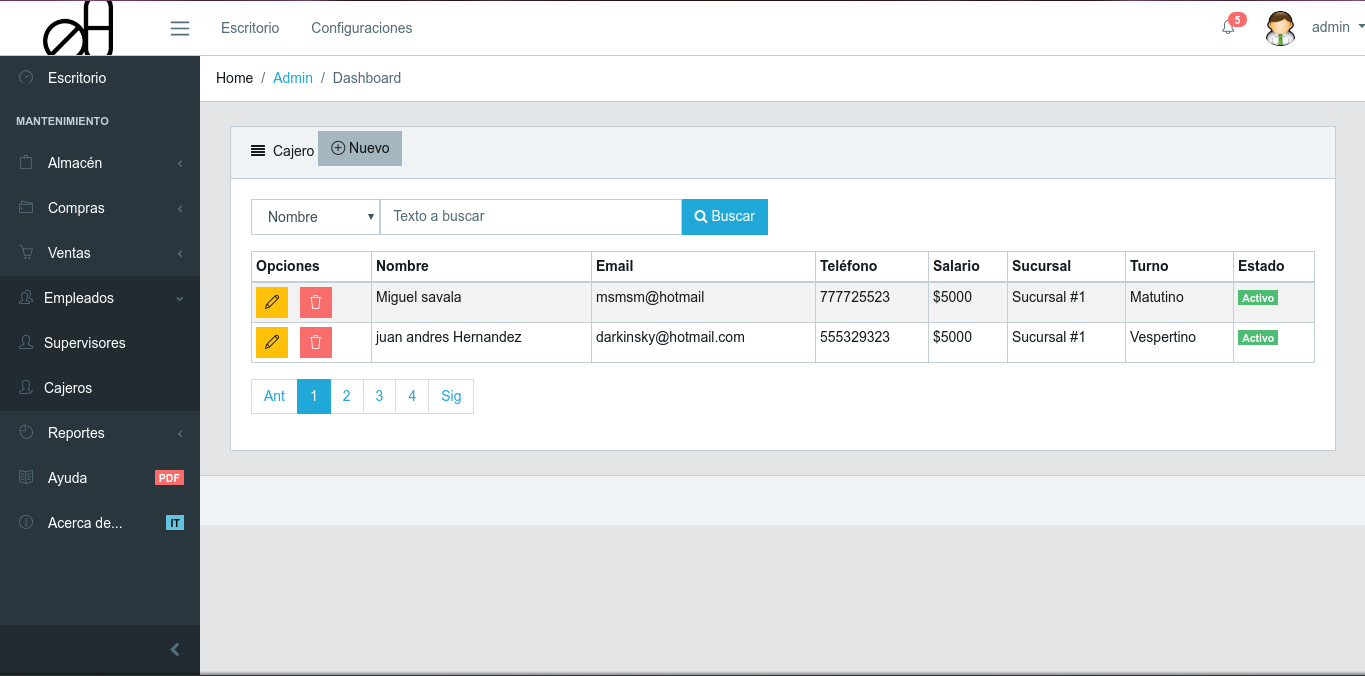
\includegraphics[width=\textwidth]{Pantallas/tablaCajeros}
		\caption{Interfaz de Usuario IU18:Tabla de Cajeros.}
	\end{center}
\end{figure}



\begin{figure}[htbp!]
	\begin{center}
	Pantalla que se muestra al realizar una venta, en esta pantalla se muestra un lista deplegable que da a escoger el tipo de cliente al que se le realiza una venta, en el campo del empleado se muestra el nombre completo del cajero que esta realizando la venta, en el campo de medicamento se esta a la espera de que se lea el medicamento desde el lector de código de barras para que se llene este campo, 
	en el desglose de medicamentos, precios y cantidad, se muestra lo que menciona el campo, se desglosa  esa información en campos de entrada que se llenan según la información del medicamento que se ha leído desde el lector de código de barras.
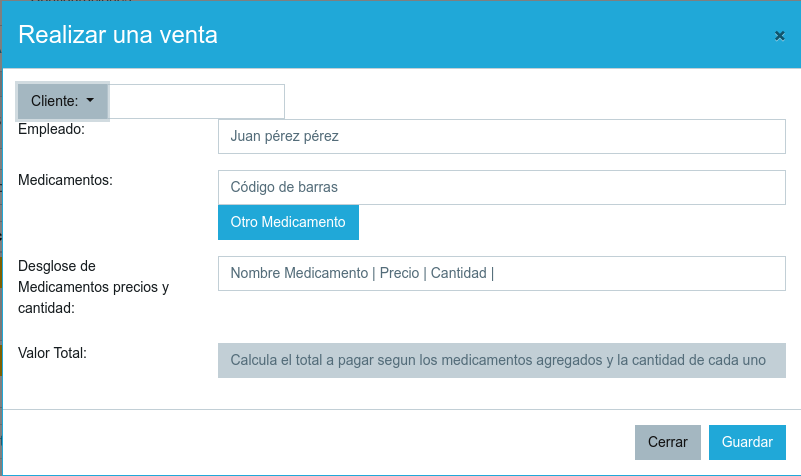
\includegraphics[width=\textwidth]{Pantallas/pantallaVentas}
		\caption{Interfaz de Usuario IU19:Pantalla Ventas.}
	\end{center}
\end{figure}

\begin{figure}[htbp!]
	\begin{center}
	En esta pantalla se muestra la infomración que se necesita guardar para poder registrar un pedido que se recibe del proveedor(un lote) donde los campos cajero y sucursal se llenan automáticamente con los datos del cajero logeado..
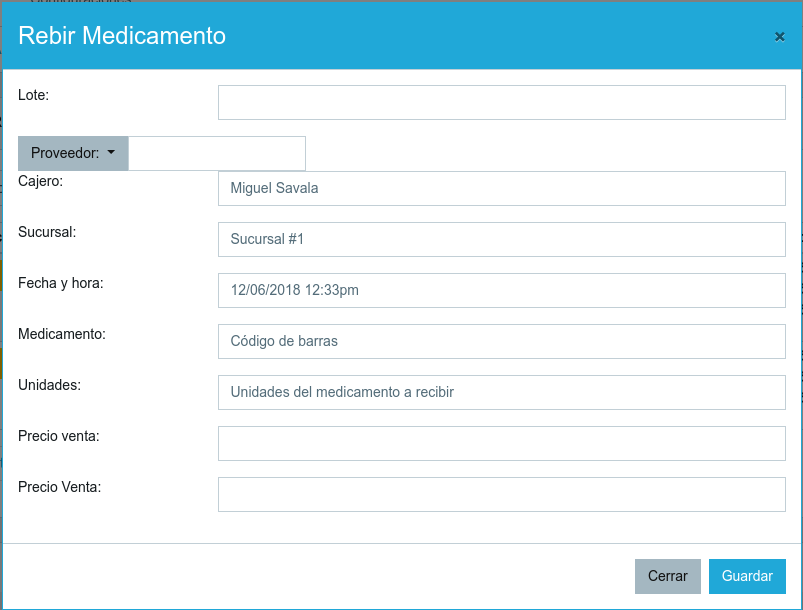
\includegraphics[width=\textwidth]{Pantallas/FormularioIngreso}
		\caption{Interfaz de Usuario IU20:Formulario Ingresos.}
	\end{center}
\end{figure}


\begin{figure}[htbp!]
	\begin{center}
	pantalla que se muestra cuando el supervisor requiere abrir caja, en esta pantalla se muestra un formulario donde el supervisor, hora y fecha  y el dinero en caja se llenan de forma automática, el dinero en caja se abre y cierra con \$1500
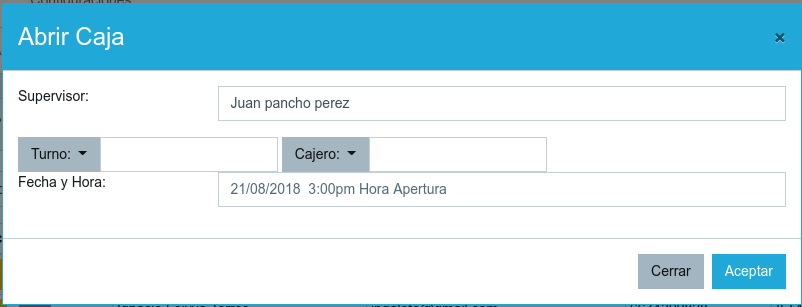
\includegraphics[width=\textwidth]{Pantallas/AbrirCaja}
		\caption{Interfaz de Usuario IU21:Abrir Caja.}
	\end{center}
\end{figure}

\begin{figure}[htbp!]
	\begin{center}
	pantalla que se muestra cuando el supervisor requiere cerrar caja, en esta pantalla son solo datos de salida pues todos son generados por el sistema.
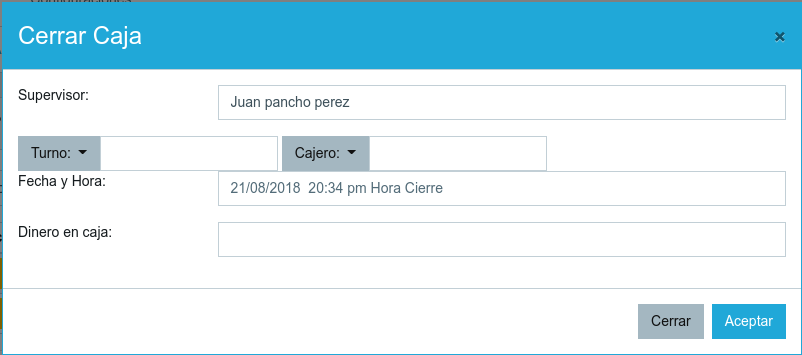
\includegraphics[width=\textwidth]{Pantallas/CerrarCaja}
		\caption{Interfaz de Usuario IU22:Cerrar Caja.}
	\end{center}
\end{figure}

\begin{figure}[htbp!]
	\begin{center}
	Pantalla que muestra la tabla de los clientes que se tienen registrados en el sistema, donde los datos de los clientes se muestran en columnas, estos datos son: NOMBRE, EMAIL, TELÉFONO, TARJETA Y EL ESTADO(ACTIVO O DESACTIVO) y se desglosan los clientes en las filas de las tablas, también están los botones de activar, desactivar y editar, aunque la opción de editar aun no esta implementada.
	se muestra un campo donde puedes hacer una búsqueda por correo y nombre.
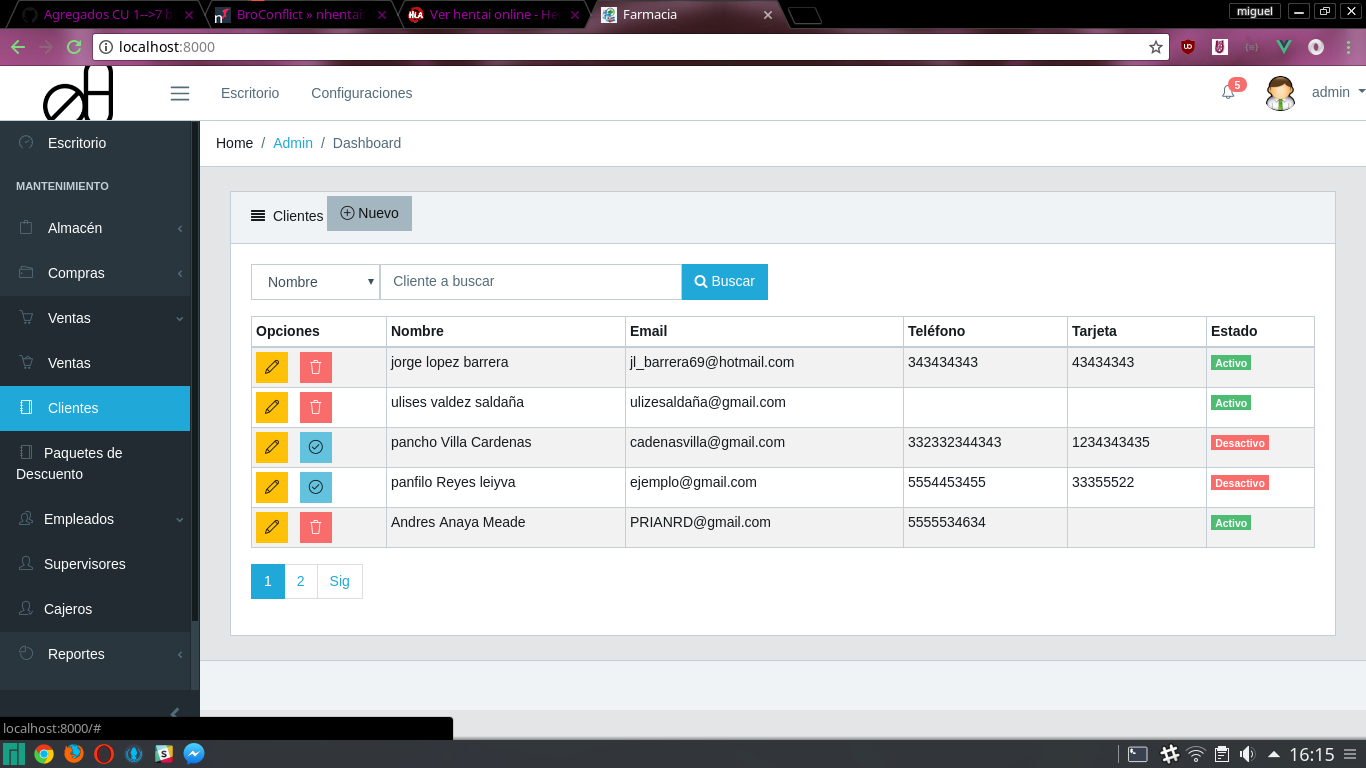
\includegraphics[width=\textwidth]{Pantallas/tablaClientes}
		\caption{Interfaz de Usuario IU23:Tabla clientes.}
	\end{center}
\end{figure}
